\documentclass[tikz,border=6pt]{standalone}
\usepackage{amsmath,amssymb}
\usepackage[T1]{fontenc}
\usetikzlibrary{
  arrows.meta,
  positioning,
  calc,
  fit,
  backgrounds,
  shapes.geometric,
  shapes.symbols,
  shadows.blur
}

% =========================
% Color Palette (NeurIPS-like)
% =========================
\definecolor{navy}{HTML}{16324F}
\definecolor{teal}{HTML}{1F9D9A}
\definecolor{softteal}{HTML}{E9F7F6}
\definecolor{softblue}{HTML}{ECF2FA}
\definecolor{orange}{HTML}{F28E2B}
\definecolor{softorange}{HTML}{FFF3E6}
\definecolor{alertred}{HTML}{D1495B}
\definecolor{slate}{HTML}{5B6770}

% =========================
% TikZ Styles
% =========================
\tikzset{
  >=Stealth,
  every node/.style={font=\small\sffamily},
  panelA/.style={
    draw=navy!70, line width=1.0pt, rounded corners=3mm, fill=softteal,
    blur shadow={shadow blur steps=6, shadow xshift=1pt, shadow yshift=-1pt}
  },
  panelB/.style={
    draw=navy!70, line width=1.0pt, rounded corners=3mm, fill=softblue,
    blur shadow={shadow blur steps=6, shadow xshift=1pt, shadow yshift=-1pt}
  },
  panelC/.style={
    draw=navy!70, line width=1.0pt, rounded corners=3mm, fill=white,
    blur shadow={shadow blur steps=6, shadow xshift=1pt, shadow yshift=-1pt}
  },
  panelD/.style={
    draw=navy!75, line width=1.0pt, rounded corners=3mm, fill=white,
    dashed, dash pattern=on 4pt off 2.3pt,
    blur shadow={shadow blur steps=6, shadow xshift=1pt, shadow yshift=-1pt}
  },
  paneltitle/.style={font=\bfseries\small, text=navy},
  state/.style={
    draw=navy!85, fill=white, rounded corners=1.8mm, line width=0.9pt,
    minimum width=1.18cm, minimum height=0.68cm, inner sep=1.5pt,
    blur shadow={shadow blur steps=4, shadow xshift=0.7pt, shadow yshift=-0.7pt}
  },
  graphnode/.style={
    circle, draw=teal!80!navy, fill=teal!18, line width=0.9pt,
    minimum size=5.0mm, inner sep=0pt
  },
  treenode/.style={
    circle, draw=teal!80!navy, fill=teal!16, line width=0.85pt,
    minimum size=4.6mm, inner sep=0pt
  },
  projector/.style={
    trapezium, trapezium left angle=76, trapezium right angle=104,
    draw=orange!90!black, fill=softorange, line width=1.0pt,
    minimum width=1.9cm, minimum height=0.95cm, inner sep=2pt,
    blur shadow={shadow blur steps=4, shadow xshift=0.8pt, shadow yshift=-0.8pt}
  },
  mlp/.style={
    draw=navy!85, fill=white, rounded corners=1.8mm, line width=0.95pt,
    minimum width=2.15cm, minimum height=0.95cm, align=center,
    blur shadow={shadow blur steps=4, shadow xshift=0.7pt, shadow yshift=-0.7pt}
  },
  targetblock/.style={
    draw=teal!85!navy, fill=softteal, rounded corners=1.8mm, line width=0.95pt,
    minimum width=2.55cm, minimum height=0.95cm, align=center,
    blur shadow={shadow blur steps=4, shadow xshift=0.7pt, shadow yshift=-0.7pt}
  },
  lossnode/.style={
    circle, draw=orange!92!black, fill=orange!20, line width=1.0pt,
    minimum size=10.2mm, inner sep=0.5pt
  },
  structedge/.style={draw=teal!75!navy, line width=1.0pt},
  structarrow/.style={-{Stealth[length=2.6mm,width=1.7mm]}, draw=teal!78!navy, line width=1.0pt},
  mainarrow/.style={-{Stealth[length=3.0mm,width=2.1mm]}, draw=navy!92, line width=1.12pt},
  treearrow/.style={-{Stealth[length=2.5mm,width=1.65mm]}, draw=navy!76, line width=0.92pt},
  depthline/.style={densely dashed, draw=navy!62, line width=1.0pt},
  extractarrow/.style={-{Stealth[length=3.2mm,width=2.2mm]}, draw=teal!88!black, line width=1.45pt, dashed},
  feedbackarrow/.style={-{Stealth[length=3.0mm,width=2.0mm]}, draw=orange!95!black, line width=1.23pt},
  auxarrow/.style={-{Stealth[length=2.6mm,width=1.7mm]}, draw=slate!70, line width=0.95pt, dashed}
}

\begin{document}
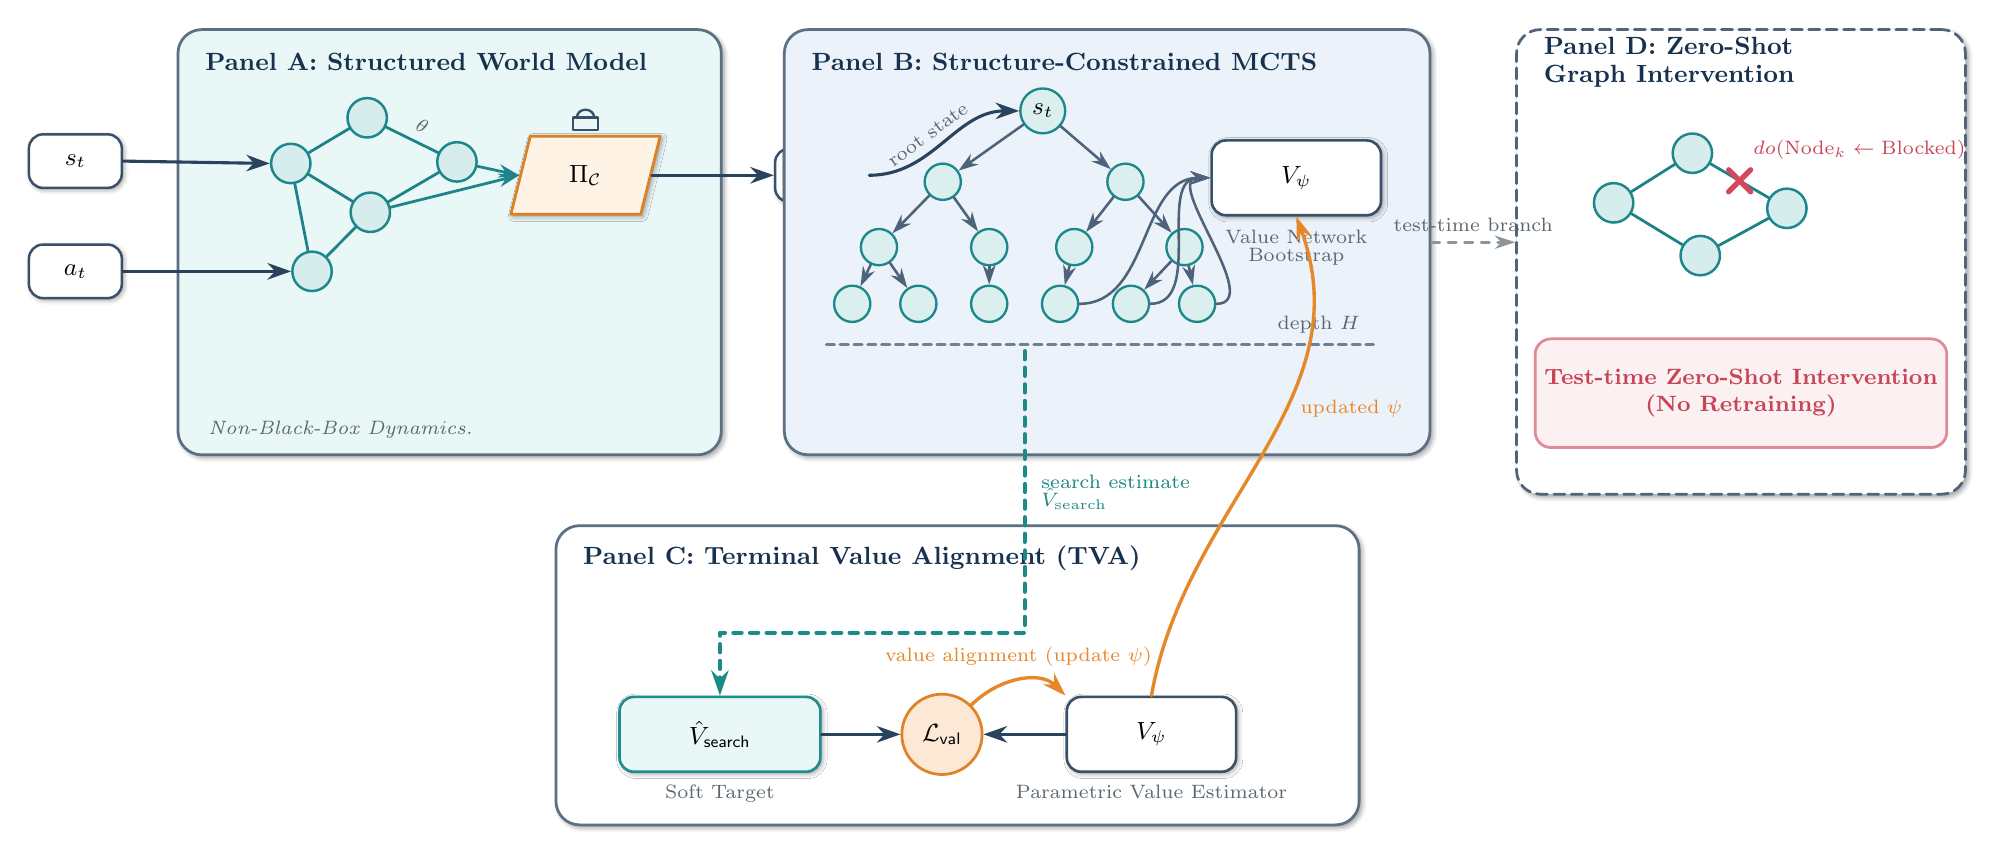
\begin{tikzpicture}[line cap=round, line join=round]

% =========================================================
% Panel A: Structured World Model
% =========================================================
\node[panelA, minimum width=6.9cm, minimum height=5.4cm, anchor=north west] (panelA) at (0,3.4) {};
\node[paneltitle, anchor=west] at ($(panelA.north west)+(0.24,-0.43)$) {Panel A: Structured World Model};

% Inputs
\node[state, anchor=east] (st) at ($(panelA.west)+(-0.68,1.03)$) {$s_t$};
\node[state, anchor=east] (at) at ($(panelA.west)+(-0.68,-0.37)$) {$a_t$};

% Structured graph (physics mechanism)
\node[graphnode] (ga1) at ($(panelA.west)+(1.45,1.00)$) {};
\node[graphnode] (ga2) at ($(panelA.west)+(2.42,1.58)$) {};
\node[graphnode] (ga3) at ($(panelA.west)+(2.46,0.38)$) {};
\node[graphnode] (ga4) at ($(panelA.west)+(3.56,1.02)$) {};
\node[graphnode] (ga5) at ($(panelA.west)+(1.72,-0.37)$) {};

\draw[structedge] (ga1) -- (ga2);
\draw[structedge] (ga1) -- (ga3);
\draw[structedge] (ga3) -- (ga4);
\draw[structedge] (ga3) -- (ga5);
\draw[structedge] (ga1) -- (ga5);
\draw[structedge] (ga2) -- node[pos=0.55, above, sloped, font=\scriptsize, text=slate] {$\theta$} (ga4);

\draw[mainarrow] (st.east) -- (ga1.west);
\draw[mainarrow] (at.east) -- (ga5.west);

% Constraint projection operator Pi_C
\node[projector, anchor=west] (proj) at ($(panelA.west)+(4.35,0.85)$) {$\Pi_{\mathcal C}$};

% Small lock icon above projector
\begin{scope}[shift={($(proj.north)+(0,0.24)$)}]
  \draw[navy!86, line width=0.85pt] (-0.16,-0.02) rectangle (0.16,-0.18);
  \draw[navy!86, line width=0.85pt] (-0.11,-0.02) arc (180:0:0.11 and 0.10);
\end{scope}

\draw[structarrow] (ga4) -- (proj.west);
\draw[structarrow] (ga3) -- (proj.west);

% Output
\node[state, anchor=west] (stp1) at ($(panelA.east)+(0.65,0.85)$) {$s_{t+1}$};
\draw[mainarrow] (proj.east) -- (stp1.west);

\node[font=\scriptsize\itshape, text=slate, anchor=west] at ($(panelA.south west)+(0.28,0.34)$) {Non-Black-Box Dynamics.};

% =========================================================
% Panel B: Structure-Bound MCTS
% =========================================================
\node[panelB, minimum width=8.2cm, minimum height=5.4cm, anchor=north west] (panelB) at (7.7,3.4) {};
\node[paneltitle, anchor=west] at ($(panelB.north west)+(0.24,-0.43)$) {Panel B: Structure-Constrained MCTS};

% Root and tree nodes
\node[treenode, minimum size=5.7mm] (r0)  at ($(panelB.north west)+(3.30,-1.05)$) {$s_t$};

\node[treenode] (b1) at ($(panelB.north west)+(2.03,-1.95)$) {};
\node[treenode] (b2) at ($(panelB.north west)+(4.35,-1.95)$) {};

\node[treenode] (c1) at ($(panelB.north west)+(1.22,-2.78)$) {};
\node[treenode] (c2) at ($(panelB.north west)+(2.62,-2.78)$) {};
\node[treenode] (c3) at ($(panelB.north west)+(3.70,-2.78)$) {};
\node[treenode] (c4) at ($(panelB.north west)+(5.10,-2.78)$) {};

\node[treenode] (l1) at ($(panelB.north west)+(0.88,-3.50)$) {};
\node[treenode] (l2) at ($(panelB.north west)+(1.72,-3.50)$) {};
\node[treenode] (l3) at ($(panelB.north west)+(2.62,-3.50)$) {};
\node[treenode] (l4) at ($(panelB.north west)+(3.52,-3.50)$) {};
\node[treenode] (l5) at ($(panelB.north west)+(4.42,-3.50)$) {};
\node[treenode] (l6) at ($(panelB.north west)+(5.26,-3.50)$) {};

\draw[treearrow] (r0) -- (b1);
\draw[treearrow] (r0) -- (b2);

\draw[treearrow] (b1) -- (c1);
\draw[treearrow] (b1) -- (c2);
\draw[treearrow] (b2) -- (c3);
\draw[treearrow] (b2) -- (c4);

\draw[treearrow] (c1) -- (l1);
\draw[treearrow] (c1) -- (l2);
\draw[treearrow] (c2) -- (l3);
\draw[treearrow] (c3) -- (l4);
\draw[treearrow] (c4) -- (l5);
\draw[treearrow] (c4) -- (l6);

% Truncation depth H
\draw[depthline] ($(panelB.north west)+(0.55,-4.02)$) -- ($(panelB.north west)+(7.50,-4.02)$);
\node[font=\scriptsize, text=slate, anchor=south east] at ($(panelB.north west)+(7.45,-4.00)$) {depth $H$};

% Bootstrap value network
\node[mlp] (vboot) at ($(panelB.north west)+(6.52,-1.90)$) {$V_\psi$};
\node[font=\scriptsize, text=slate, anchor=north, align=center] at ($(vboot.south)+(0,-0.05)$) {Value Network\\[-0.5ex]Bootstrap};

\draw[treearrow] (l4) to[out=0,in=180] (vboot.west);
\draw[treearrow] (l5) to[out=0,in=180] (vboot.west);
\draw[treearrow] (l6) to[out=0,in=180] (vboot.west);

% Main flow A -> B
\draw[mainarrow] (stp1.east) to[out=0,in=180] node[pos=0.45, above, sloped, font=\scriptsize, text=slate] {root state} (r0.west);

% =========================================================
% Panel C: Terminal Value Alignment (TVA)
% =========================================================
\node[panelC, minimum width=10.2cm, minimum height=3.8cm, anchor=north west] (panelC) at (4.8,-2.9) {};
\node[paneltitle, anchor=west] at ($(panelC.north west)+(0.24,-0.43)$) {Panel C: Terminal Value Alignment (TVA)};

\node[targetblock] (vsearch) at ($(panelC.west)+(2.10,-0.75)$) {$\hat{V}_{\text{search}}$};
\node[font=\scriptsize, text=slate, anchor=north] at ($(vsearch.south)+(0,-0.03)$) {Soft Target};

\node[lossnode] (loss) at ($(panelC.west)+(4.92,-0.75)$) {$\mathcal{L}_{\text{val}}$};

\node[mlp] (vpsi) at ($(panelC.west)+(7.58,-0.75)$) {$V_\psi$};
\node[font=\scriptsize, text=slate, anchor=north] at ($(vpsi.south)+(0,-0.03)$) {Parametric Value Estimator};

\draw[mainarrow] (vsearch.east) -- (loss.west);
\draw[mainarrow] (vpsi.west) -- (loss.east);

% Alignment + update loop
\draw[feedbackarrow] (loss.north east) to[out=45,in=135]
  node[pos=0.5, above=0.3ex, font=\scriptsize, text=orange!95!black] {value alignment (update $\psi$)} (vpsi.north west);

% Updated parameters back to bootstrap network in Panel B
\draw[feedbackarrow] (vpsi.north) to[out=80,in=-70]
  node[pos=0.6, right=2pt, font=\scriptsize, text=orange!95!black] {updated $\psi$} (vboot.south);

% Search statistics extraction from tree to TVA
\coordinate (treeStat) at ($(l3)!0.5!(l4)$);
\coordinate (treeStat) at ($(treeStat) +(0,-0.6)$);
\draw[extractarrow] (treeStat) |- 
  node[pos=0.25, right=2pt, font=\scriptsize, text=teal!85!black, align=left] {search estimate\\[-0.5ex]$\hat{V}_{\text{search}}$}
  ($(vsearch.north)+(0,0.8)$) -- (vsearch.north);

% =========================================================
% Panel D: Zero-Shot Graph Intervention (Inset)
% =========================================================
\node[panelD, minimum width=5.7cm, minimum height=5.9cm, anchor=north west] (panelD) at (17.0,3.4) {};
\node[paneltitle, anchor=west, align=left] at ($(panelD.north west)+(0.24,-0.43)$) {Panel D: Zero-Shot\\[-0.2ex]Graph Intervention};

% Small causal/physical graph
\node[graphnode] (d1) at ($(panelD.west)+(1.25,0.75)$) {};
\node[graphnode] (d2) at ($(panelD.west)+(2.25,1.38)$) {};
\node[graphnode] (d3) at ($(panelD.west)+(2.35,0.08)$) {};
\node[graphnode] (d4) at ($(panelD.west)+(3.45,0.68)$) {};

\draw[structedge] (d1) -- (d2);
\draw[structedge] (d1) -- (d3);
\draw[structedge] (d3) -- (d4);
\draw[structedge] (d2) -- (d4);

% Intervention marker on one edge
\path (d2) -- (d4) coordinate[midway] (cutpt);
\draw[alertred, line width=1.9pt] ($(cutpt)+(-0.14,0.14)$) -- ($(cutpt)+(0.14,-0.14)$);
\draw[alertred, line width=1.9pt] ($(cutpt)+(-0.14,-0.14)$) -- ($(cutpt)+(0.14,0.14)$);

\node[font=\scriptsize, text=alertred!95!black, anchor=west] at ($(cutpt)+(0.05,0.40)$)
{$do(\text{Node}_k \gets \text{Blocked})$};

% Emphasis text box
\node[
  draw=alertred!65, fill=alertred!8, rounded corners=2mm, line width=1.0pt,
  minimum width=4.85cm, minimum height=1.38cm, align=center,
  text=alertred!95!black, font=\bfseries\footnotesize
] at ($(panelD.south)+(0,1.30)$) {Test-time Zero-Shot Intervention\\(No Retraining)};

% Independent branch connector
\draw[auxarrow] ($(panelB.east)+(0,0)$)
  -- node[above, font=\scriptsize, text=slate] {test-time branch}
  ($(panelD.west |- panelB.east)+(0,0)$);

\end{tikzpicture}
\end{document}
